\chapter{Формализация задачи}
\section{Описание задачи}
Задачи классификации изображений растений заключается в определении вида или подвида растения по его изображению. Несмотря на то, что существуют различные решения задачи, можно выделить общий подход, который состоит из 4 этапов, приведённых на изображении~\ref{general}: захват изображения, предобработка изображений, извлечение признаков, использование методов классификации.

Для захвата изображения используются цифровые камеры с целью получения 2D представления, однако при решении задачи классификации могут быть использованы и менее распространённые средства, такие как тепловизионная камера, например, для сбора 2D-изображений апельсинов~\cite{ref12} и лазерный сканер для получения 3D-изображений, когда необходима полная информация о растении, как в статье "Классификация органов растений на основе поверхностных характеристик из трёхмерных облаков точек, полученных с помощью лазерного сканирования, для
фенотипирования растений"~\cite{ref15}.

Этап предобработки изображений включает в себя следующие шаги: переориентация изображения, кадрирование изображения, преобразование изображения в оттенки серого, после чего выполняется преобразование в двоичное изображение, удаление шума, растяжение контраста и инверсия порогового значения~\cite{ref19}. Исследование в~\cite{ref20} показало, что для извлечения особенностей листьев изображение листа делится на 2/4 части, а не извлекается целиком.

Этап извлечения признаков изображения имеет ключевое значение в задаче классификации, поскольку именно на основе полученных признаков модель будет принимать решение в пользу того или иного класса. Для извлечения текстурных признаков используются некоторые статистические меры, такие как матрица совместного появления цветов (CCM), матрица пространственной зависимости от уровня серого (SGLDM), матрица совместного появления уровней серого (GLCM), локальные бинарные паттерны (LBP). Существующие системы и методы распознавания растений зависят от цвета, размера, формы и текстуры изображения листа.

Этап классификации представляет собой методы, с помощью которых и определяется класс объекта на изображении. Нередко встаёт задача о подборе оптимальной пары - метода извлечения признаков и классификации. 

В рамках данной работы основное внимание уделено именно методам извлечения признаков и классификации. Этап захвата изображений не рассматривается в виду использования датасета, описанного в ограничениях.

\begin{figure}[h]
	\centering
	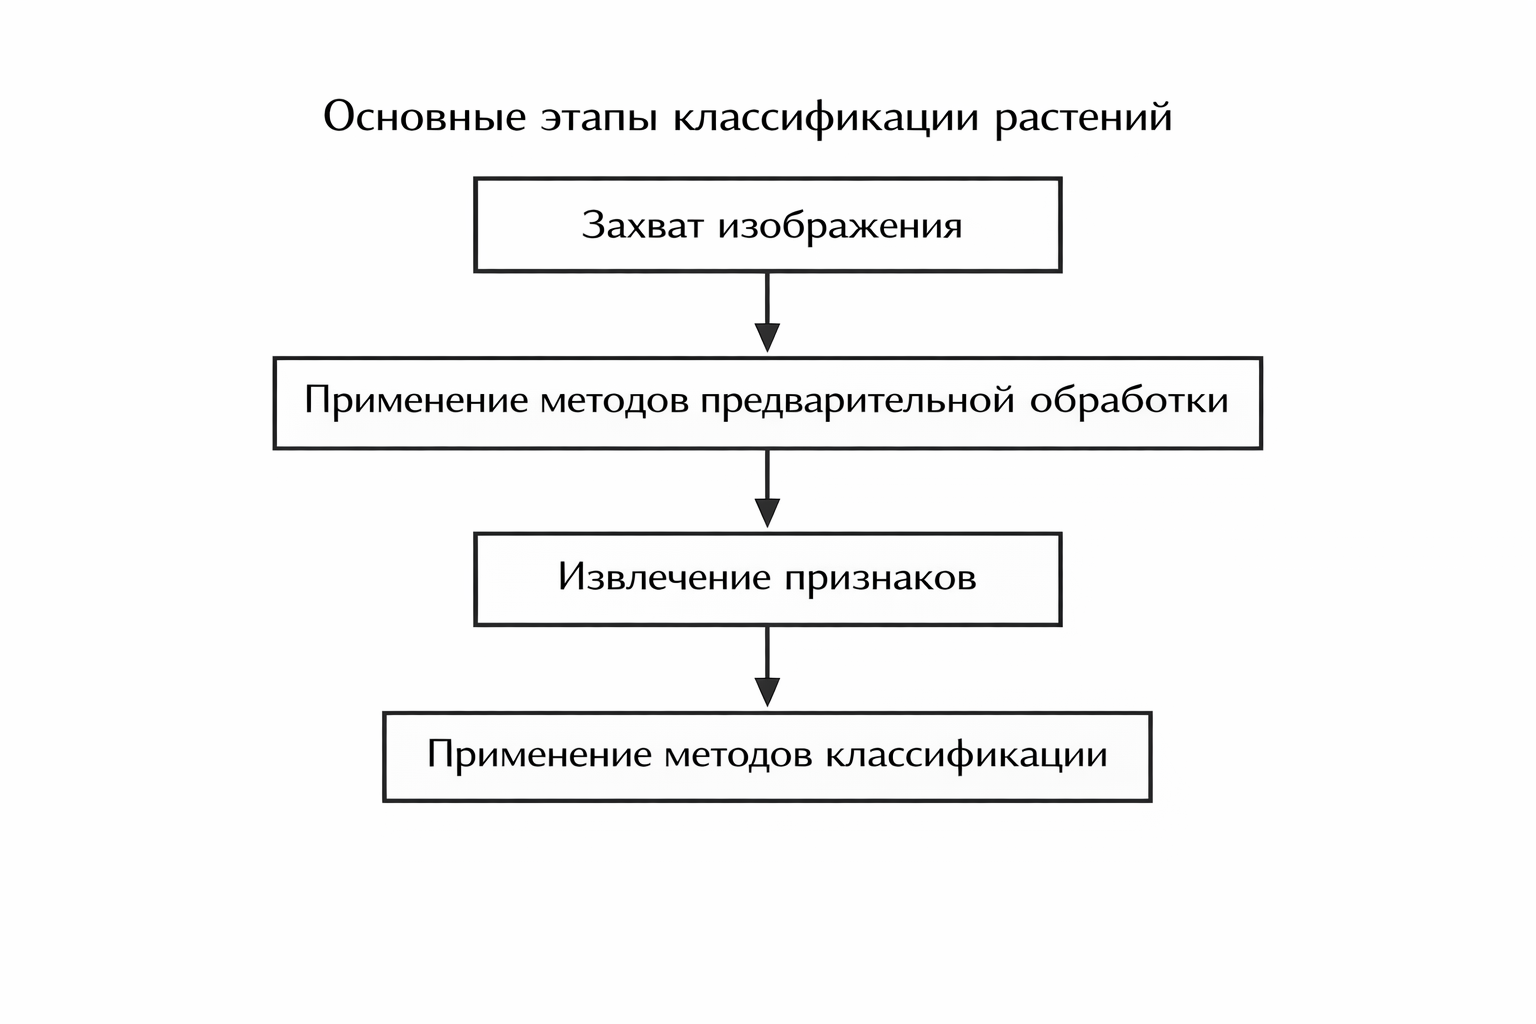
\includegraphics[width=\linewidth]{inc/img/general.png}
	\caption{Основные этапы классификации растений}
	\label{general}
\end{figure}
\clearpage
\section{Формализованная постновка задачи}
Функциональная модель представлена на рисунка~\ref{general_task}~-~\ref{details_task}.
\begin{figure}[h]
	\centering
	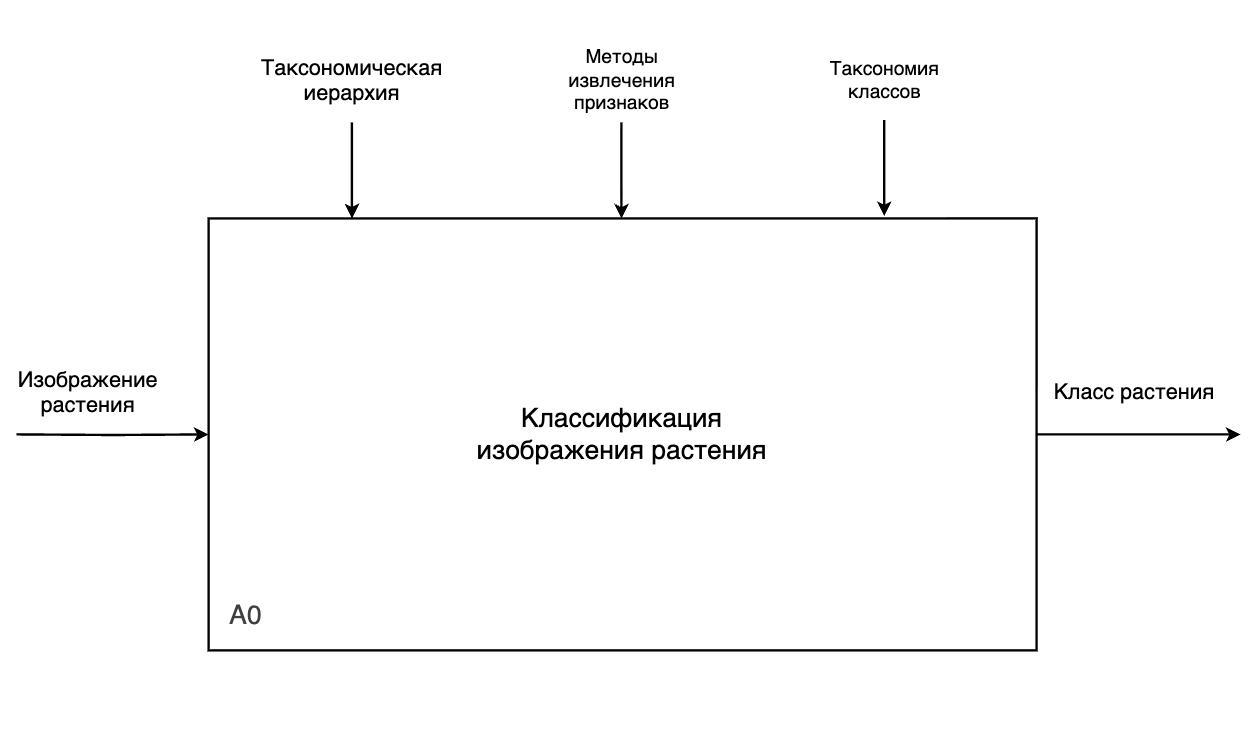
\includegraphics[width=0.7\linewidth]{inc/img/A0.png}
	\caption{Функциональная модель}
	\label{general_task}
\end{figure}

\begin{figure}[h]
	\centering
	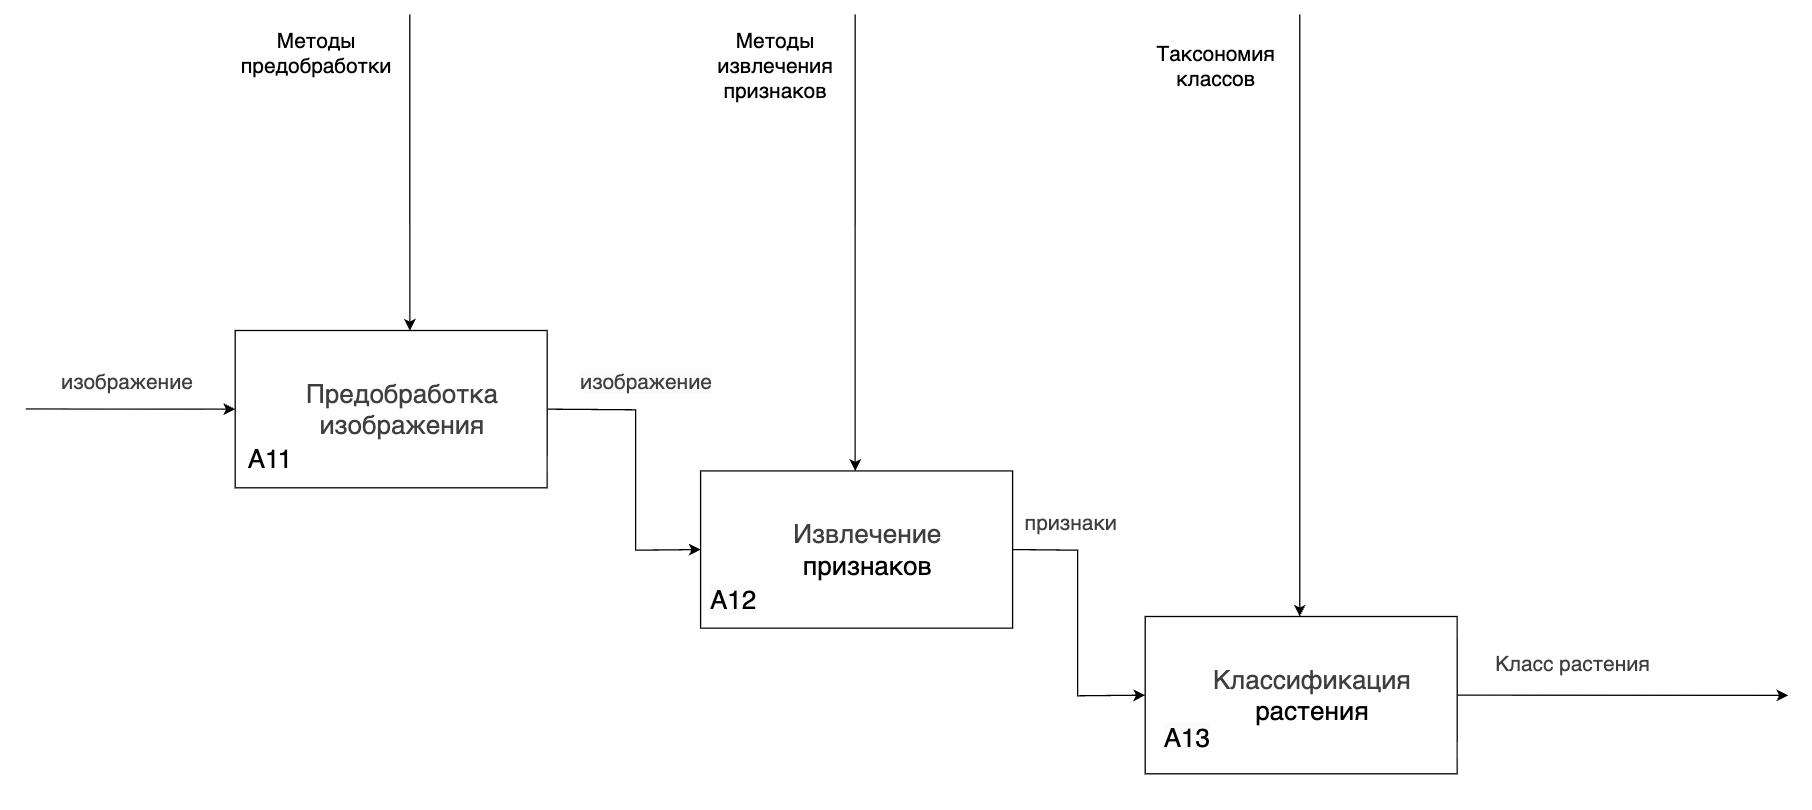
\includegraphics[width=\linewidth]{inc/img/A1.png}
	\caption{Функциональная модель}
	\label{details_task}
\end{figure}
\clearpage
%В качестве демонстрации общего подхода приведён псевдокод %для решения задачи классификации изображения на %листинге~\ref{example_algorithm}. 

%\begin{algorithm}[H]
%	\caption{Классификация изображений растений с использованием глубокого обучения}
%	\label{example_algorithm}
%	\begin{algorithmic}[1]
	%		\State \textbf{Вход:} обучающая выборка $X \in \mathbb{R}^{m \times n}$, метки классов $Y$, число слоёв $l$
	%		\State \textbf{Выход:} обученные веса модели или предсказанные метки классов
	%		\State Инициализировать веса модели малыми случайными значениями
	%		\State Задать скорость обучения $\alpha$, максимальное число эпох, порог ошибки
	%		\State Выполнить предварительную обработку данных: нормализация, изменение размера, one-hot кодирование меток
	%		\State Установить epoch $\leftarrow 0$, loss $\leftarrow \infty$
	%		\While{epoch $<$ max\_epochs и loss $>$ error\_threshold}
	%		\State epoch $\leftarrow$ epoch $+ 1$
	%		\For{всех мини-пакетов $(x_i, y_i)$ в обучающей выборке}
	%		\State \textbf{Прямой проход:}
	%		\State Пропустить входные данные $x_i$ через модель $f_{\theta}$ для получения предсказания $\hat{y}_i = f_{\theta}(x_i)$
	%		\State Модель $f_{\theta}$ может включать свёрточные слои, блоки внимания, нормализацию и нелинейности в зависимости от архитектуры
	%		\State Вычислить предсказание $\hat{y}_i$
	%		\State \textbf{Вычисление функции потерь:} вычислить $L(y_i, \hat{y}_i)$ (например, кросс-энтропию)
	%		\State \textbf{Обратное распространение ошибки:}
	%		\State Вычислить градиенты $\nabla_{\omega} L$
	%		\State Обновить веса: $\omega \leftarrow \omega - \alpha \cdot \nabla_{\omega} L$
	%		\EndFor
	%		\State Вычислить среднее значение функции потерь для текущей эпохи
	%		\State При необходимости выполнить оценку на валидационной или тестовой выборке
	%		\EndWhile
	%		\State \textbf{вернуть} обученную модель или предсказанные метки классов
	%	\end{algorithmic}
%\end{algorithm}
\section{Ограничения}
К ограничениям решения задачи относятся качество исходных изображений, и объем исходных данных, которые напрямую влияют на точность классификации, а также визуальная схожесть между растениями одного класса. 

Для сравнения методов используется датасет PlantClef 2015~\cite{ref1100}, поскольку данный датасет включает фотографии, собранные фотографами в разных точках мира, различных условиях. Вдобавок, данный датасет несбалансирован и имеет ограниченное количество изображений для некоторых видов, а также для него предопределен тестовый набор, что позволяет сравнивать методы, использующие данный датасет.

